\section{ATLAS Detector Upgrade}

\subsection{High Luminosity Large Hadron Collider - HL-LHC}
The Large Hadron Collider (LHC), run by CERN at the Franco-Swiss border near Geneva, is a circular accelerator with 27 km of acceleration pipes, is the largest scientific instrument ever designed and built for scientific research. Successfully commissioned in March 2010 for proton-proton collision with a 7 GeV centre-of-mass energy.\\
The LHC is pusshing the limits of human knowledge, enabling physicist to go beyond Standar Model (SM): the enigmatic Higgs boson, mysterious Dark Matter and the world of supersymetry are just three of the long-awaited mysterous that the LHC will unveil. The announcement given by CERN on 4 July 2012 about the discovery of new boson at 125-126 GeV, almost certainly the long awaited Higgs particle, is the first fundamental discovery, hopefully the first of a series, that the LHC can deliver.\\
Such discovery was thanks to the different detectors located on the four interaction points; ALICE, LHCb, CMS and ATLAS. This last one is the detector where our university is taking part.\\
\begin{figure}[ht]
		\centering
		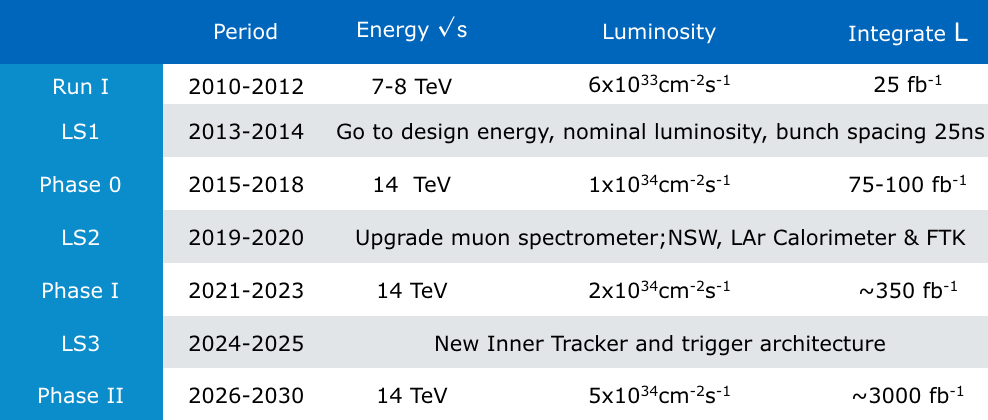
\includegraphics[width=0.7\textwidth]{LHC_program_table.png}
		\caption{LCH Schedule}\label{fig:a}
\end{figure}
\par
CONTINUE WITH LHC UPGRADE and GOALS

\subsection{ATLAS Detector}
The ATLAS detector it is a general-purpose detector, designed to explore proton-proton colissions at center of mass up to $\sqrt{s}=$14 GeV. Looking for.... \par
Such energy has been achived from 2015 and successfuly working with a luminosity of 1x10$^{34}$cm$^{-2}s^{-1}$ from 2016.\\

Describe ATLAS detector and its part, together with the problem faced by now.\par


ENDING WITH THE FAKE TRIGGERS AND PROBLEMS FOR LOW PT.\par 



\subsection{New Small Wheel}

In manner to fullfill the LHC program (in fig.\ref{fig:a}), and in order to benefit from the expected high luminosity performance that will be provided by the Phase-I upgraded LHC, 
the first station of ATLAS muon end-cap system (Small Wheel, SW) will need to be replaced. 
The New Small Wheel (NSW) will have to operate in a high background radiation region (upto 15kHz/cm$^2$) while reconstructing muon tracks with high precision as well as furnishing 
information for the Level-1 trigger. These performance criteria are demanding. In particular, the precision reconstruction of tracks for offline analysis requires a spatial resolution about 100 $\mu$m, and the Level-1 trigger track segments have to be reconstructed online with an angular resolution of approximately 1mrad. The NSW will have to chamber technologies, one primarily devoted to the Level-1 trigger function (small-strip Thin Gap Chambers, sTGC) and one dedicated to precision tracking (Micromegas detectors, MM). The sTGC are primarily deployed for triggering given their single bunch corssing identification capability. The MM detectors have exceptional precision tracking capabilities due to their small gap (5mm) and strip pitch (approximately 0.5mm). Such a precision is crucial to maintain the current ATLAS muon momentum resolution in the high background environment of the upgraded LHC. The MM chambers can, at the same time, confirm the existence of a track segments found by the muon end-cap middle station (Big Wheels) online. The sTGC also has the ability to measure offline muon tracks with good precision, so the sTGC-MM chamber technology combination forms a fully redundant detector system for triggering and tracking both for online and offline functions. This detector combination has been designed to be ablo to also provide excellente performance for the eventual High Luminosity LHC upgrade.\par 



\section{Small-strip Thing Gap Chamber}

The sTGC detector it is a multiwire proportional chamber (MWPC) working in a high gain mode with a cathode-anode pitch smaller than the anode-anode pitch, mostly based on the design of the Thin Gap Chamber\cite{tgc}, with thinner strips as the main improvement. The TGC tecnology has been used since 1988 in OPAL experiment and currently are part of the the muon spectrometer in ATLAS. \\
	This new  chamber has the advantage of having a 3.2mm strip width compare to the 5-6 mm from the previous TGC, that is why it is called small strip Thin Gap Chamber (sTGC from now on).\\ 
	The size of the strips has been choosen to cope up with the precision resolution require for the NSW (explained before), where it has to be better than 100 $\mu$m and provide a reponse with a few nanoseconds. For this purpose, chambers with different strips sizes has been build and test under pion beams, chosed the 3.2mm has the best option\cite{stripwidth}. \par
%-------- sTGC Explanation -------

The sTGC is made of two cathods planes, one with copper strips and the other with pads, each cathode plane is made of FR4 with 1.6mm of thickness, where  100 $\mu$m of copper is etched for strips (pads) and then pressed with a 100 $\mu$m of FR4 over it to provide a homogenous surface so it can be sprayed with graphite to achieve 100-200 k$\Omega / \square$ (1 M$\Omega/\square$ for TGC). The anodes are golden tungsten wires of 50 $\mu$m diameter, distributed at 1.8 mm  between each other. The gas gap (2.8mm) is filled with a mixture of CO$_2$ and n-pentane in proportion 55:45 respectively both strongly quenching gases that provide a high amplification factor and relatively low sensitivity to mechanical variations.\\  


%----------- sTGC mode picture -----

\begin{figure}[h]
		\centering
		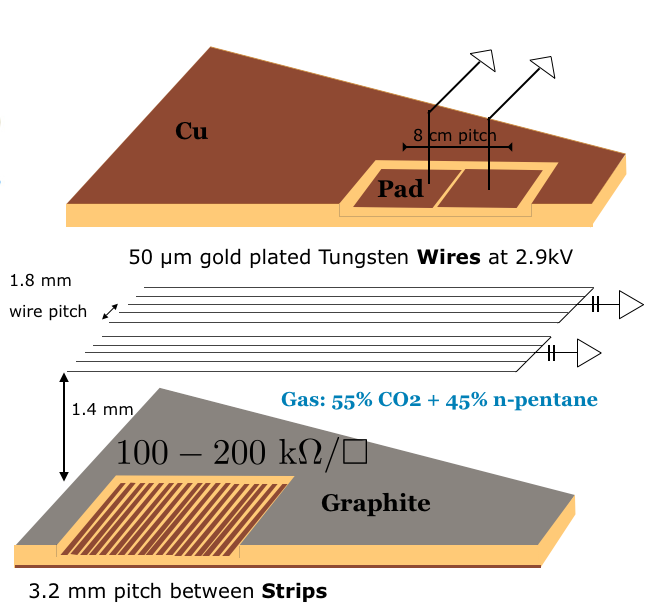
\includegraphics[width=0.5\textwidth]{sTGC_layout.png}
		\caption{Single plane sTGC}\label{fig:sTGC}
\end{figure}

A MWPC is a relativetely old technology, its succesfuly introduction to detector system in 1968 gave the Nobel prize to George Charpak in 1922. This device has been a major ingrediente in detector systems since it can achieve spatial resolutions of 500 $\mu$m or less, and has typical time resolution of about 30 ns.\\
\begin{itemize}
\item Explicar geometria del sTGC, gas gap y wire pitch.
\item explicar eleccion de gas
\item voltaje de operacion.
\item resitividad del graphito y para que usamos grafito.
\item Que es lo moderno de este detector...
\end{itemize}


\section{Construction process}
Cathode production and how we achieve the resolution requeride for this.\\
Clean cathode\\
Sprayed process\\
Achieve the proper superficial resistivity\\
glue internal parts\\
Winding wires, soldered and clean afterwards\\
test wires under hv\\
Close chamber and filled with CO$_2$, no sparks must found\\
glue chamber\\
Thickness measurments\\
Repeat process till get 4 modules\\
Overall thickness measurements and pin position check\\


\section{Gain uniformity measurements}

One of the Quality Acceptance and Quality Control (QA/QC) is to test each single plane under x-rays to check the homogenity of the detector on different spots, looking for construction issues that may cause some high variation on the signal for a single hit. To provide such test we use a x-ray gun placed in a robotic arm (KUKA) and move it through different position of the chamber, going from active to non active areas covering the full size of the detector, recording at the same time the current draw from the High Voltage power supply.\\
What can affect the gain?\\
Why we use X-rays?\\

\subsection{Setup}
Provide explanation of setup and posterior details of instruments.\\

\begin{itemize}
\item X-ray source: Mini-X gun with photons of  50 keV and flux of  45 $\mu$A
\item Collimator: 5º.
\item Distance from source: 2.5 $\pm$ 0.3 cm. Spot size: 2 $\pm$ 0.26 mm.
\item KUKA arm; giving vertical steps:1.5 cm, horizontal steps: 5 cm.
\item HV power supply: 50 nA resolution. Sampling rate: 1 sample/s.
\end{itemize}


\subsection{Results}

\begin{figure}[h]
	\centering
	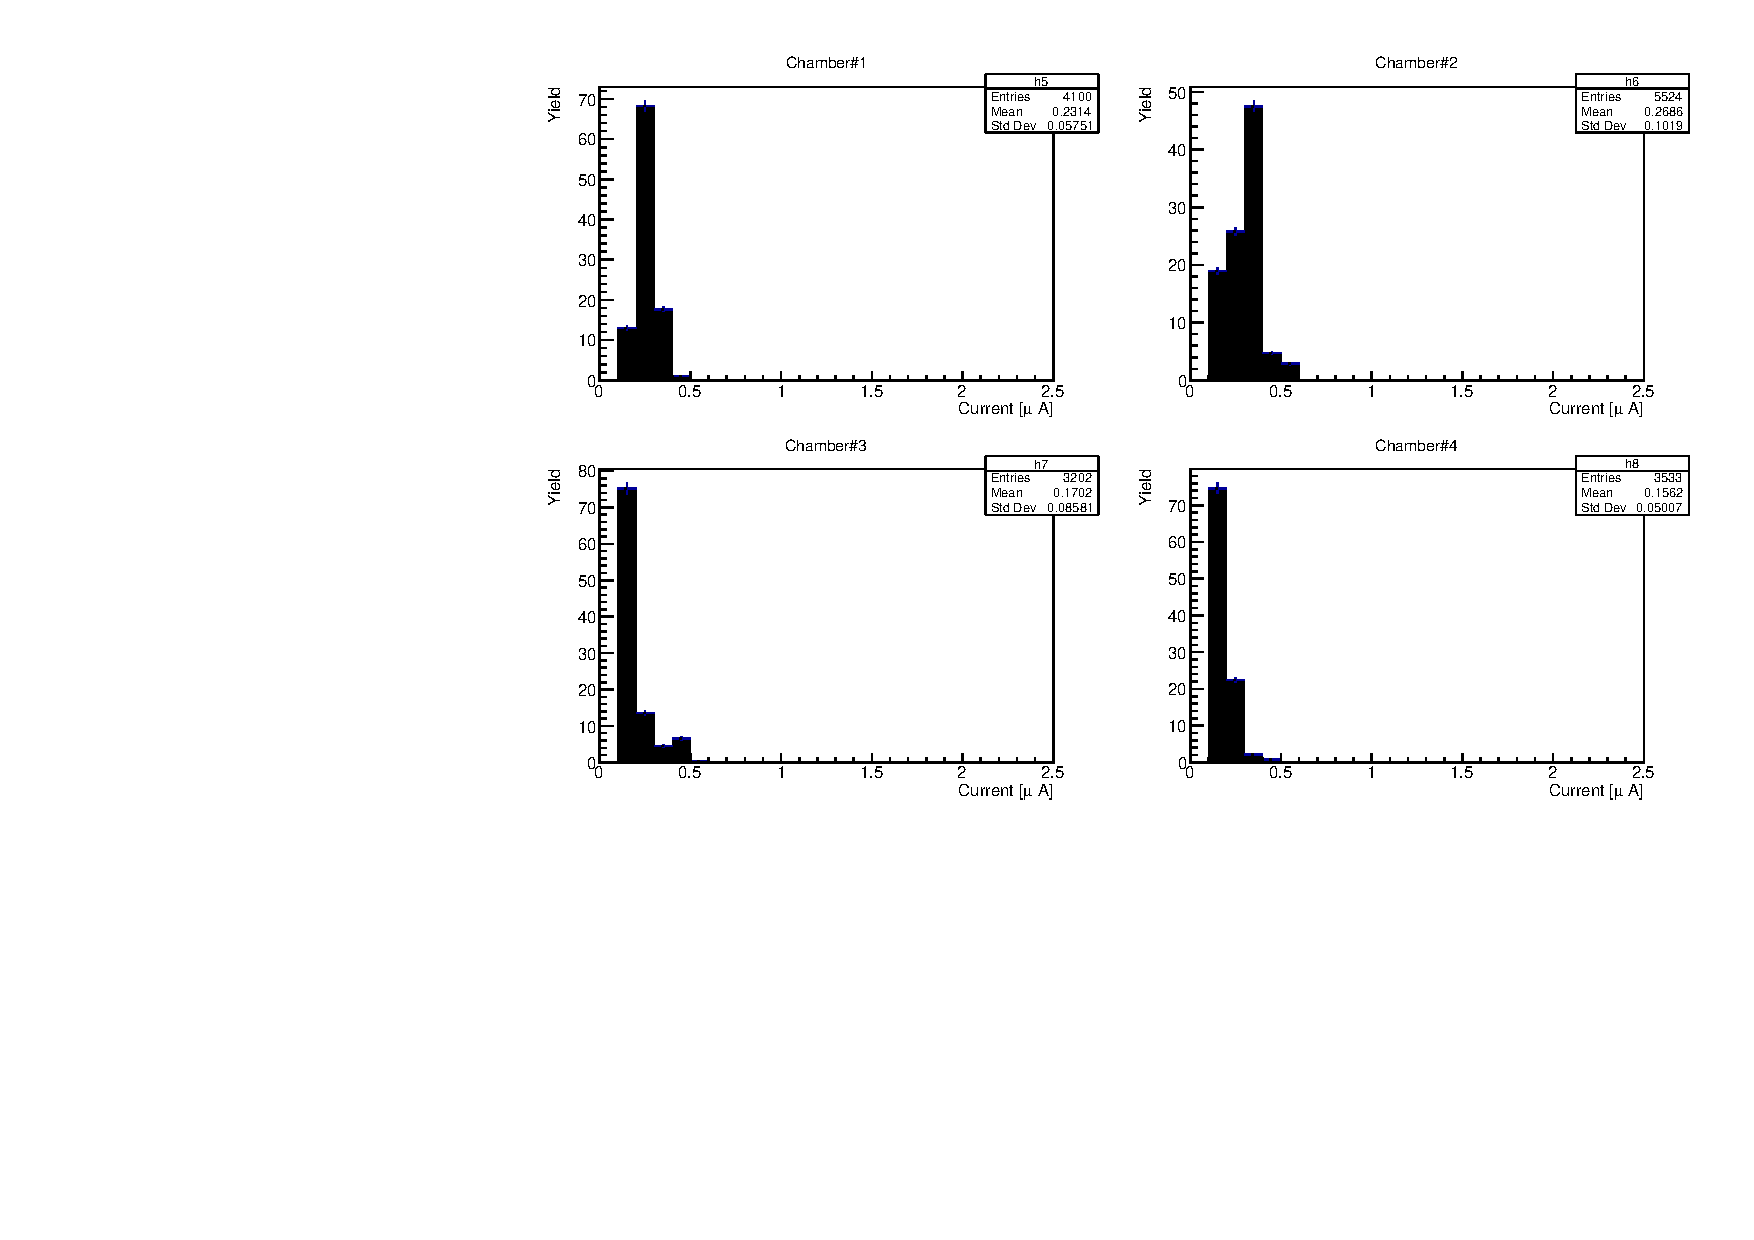
\includegraphics[width=0.7\textwidth]{uniformity_2500.pdf}
	\caption{Current draw from PS at 2500V}\label{fig:2500V}
\end{figure}

\begin{figure}[h]
	\centering
	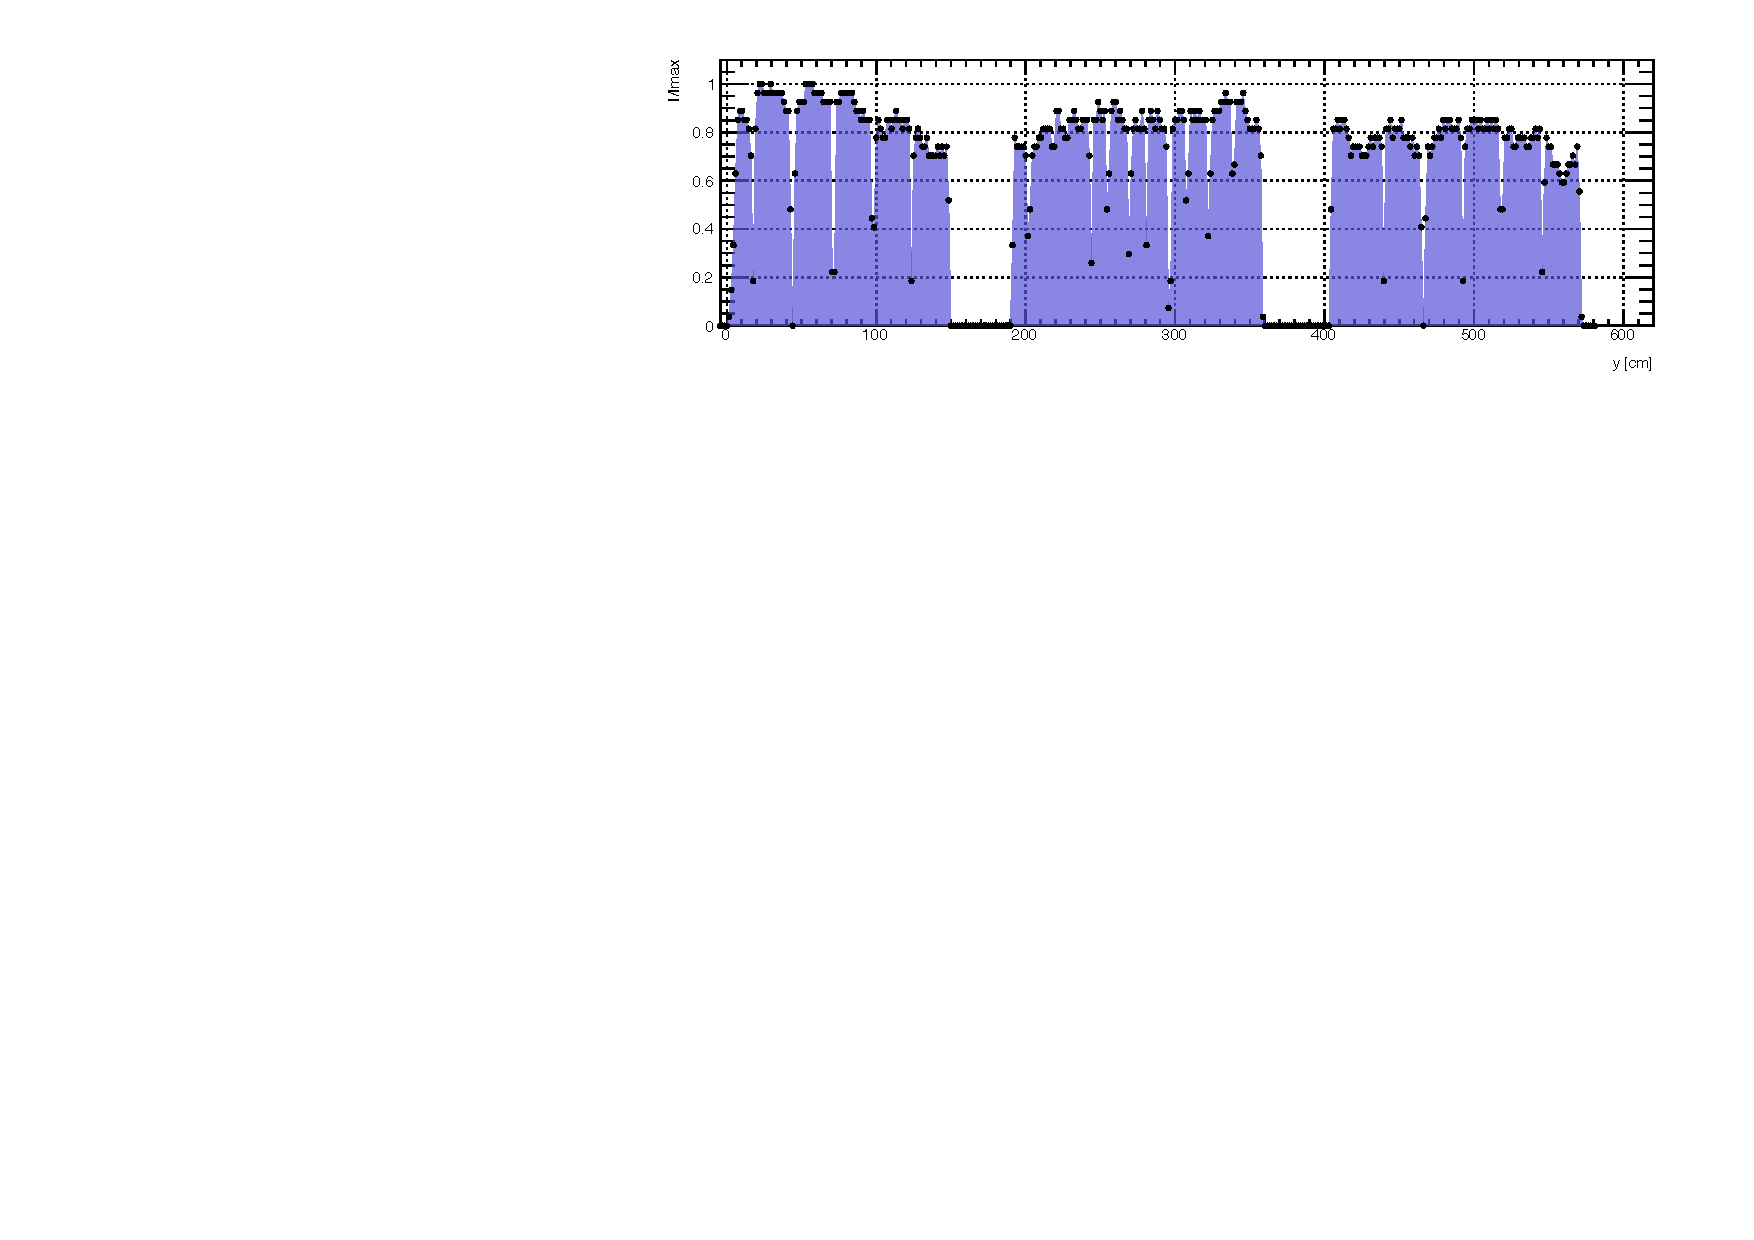
\includegraphics[width=0.7\textwidth]{uniformity_2900.pdf}
	\caption{Current draw from PS at 2900V}\label{fig:2900V}
\end{figure}


\section{Test under high rate}


\section{Spatial resolution strips}

\section{Charge sharing between pads}

\section{summary}
